% Slides for 2025-08-19
% To create a slide, use the following:
% \begin{frame}{TITLE}
%     BODY
% \end{frame}

% To create a slide with a bullet list, use the following:
% \begin{frame}{TITLE}
%     \begin{itemize}
%         \item ITEM 1
%         \item ITEM 2
%     \end{itemize}    
% \end{frame}

% To create a slide with numbered list, use the following:
% \begin{frame}{TITLE}
%     \begin{enumerate}
%         \item ITEM 1
%         \item ITEM 2
%     \end{enumerate}
% \end{frame}

% To create a slide with a graphic:
% 1. Add the graphic to this folder (named picture.png)
% 2. Use the following:
% \begin{frame}{TITLE}
%     \centering
%     \includegraphics[height=0.7\textheight,width=0.7\textwidth,keepaspectratio]{picture.png}
% \end{frame}

% To create a slide with two columns, use the following:
% \begin{frame}{TITLE}
%     \begin{columns}
%         \begin{column}{0.5\textwidth}
%             COLUMN 1 BODY
%         \end{column}
%         \begin{column}{0.5\textwidth}
%             COLUMN 2 BODY
%         \end{column}
%     \end{columns}
% \end{frame}

\begin{frame}{ML Team Agenda}
    \begin{itemize}
        \item Knowledge Graph w/ Temporal + Template Matching
        \item Autoencoders
        \item Clustering
        \item D3.JS Visualization
        \item Future Steps
    \end{itemize}
\end{frame}

\begin{frame}{Knowledge Graph w/ Temporal + Template Matching}
    \begin{itemize}
        \item 
    \end{itemize}
\end{frame}
\begin{frame}{Autoencoders}
    \centering
    \begin{figure}
        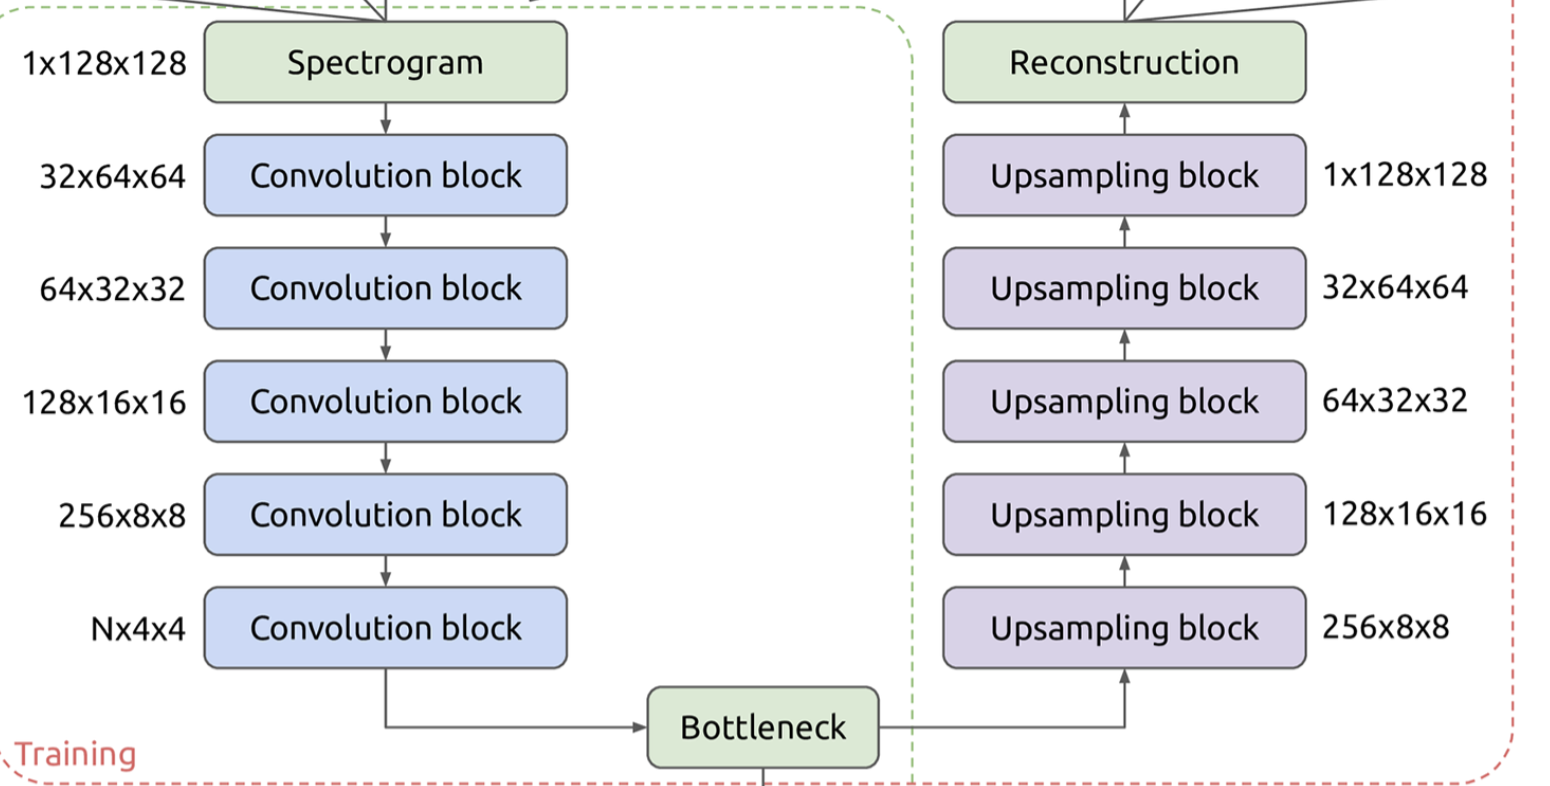
\includegraphics[height=\textheight,width=\textwidth,keepaspectratio]{images/architecture.png}
        \caption{Model Architecture, adapted from Best et. al. 2023}
    \end{figure} 
\end{frame}
            

\begin{frame}{Autoencoders as Unlabeled Embedders}
    \begin{figure}
        \begin{columns}
            \begin{column}{0.5\textwidth}
                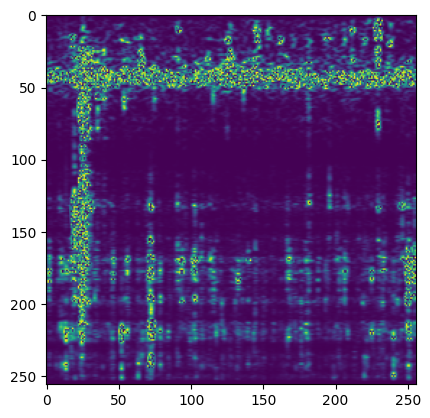
\includegraphics[height=\textheight,width=\textwidth,keepaspectratio]{images/pre_mel.png}
            \end{column}
            \begin{column}{0.5\textwidth}
                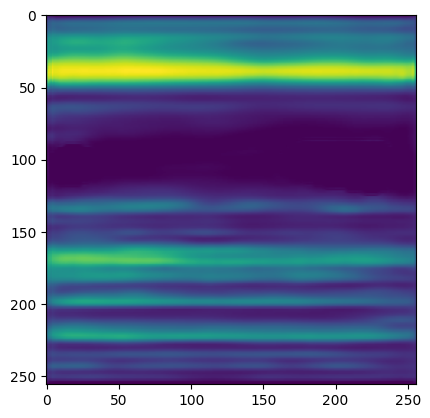
\includegraphics[height=\textheight,width=\textwidth,keepaspectratio]{images/post_mel.png}
            \end{column}
        \end{columns}
        \caption{Autoencoder melspectrogram pre (left) and post (right) processing }
    \end{figure}
\end{frame}

\begin{frame}{Autoencoder Clustering}
    \centering
    \begin{figure}
        \begin{columns}
            \begin{column}{0.5\textwidth}
                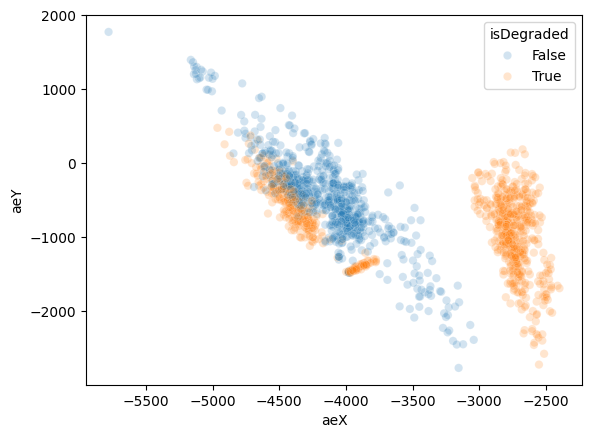
\includegraphics[height=\textheight,width=\textwidth,keepaspectratio]{images/auto_clustering_labeled.png}
            \end{column}
            \begin{column}{0.5\textwidth}
                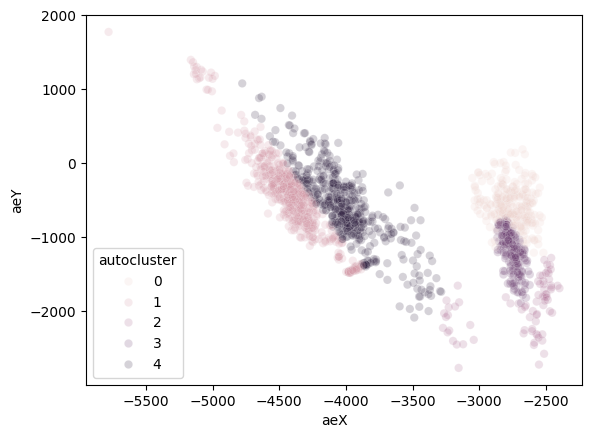
\includegraphics[height=\textheight,width=\textwidth,keepaspectratio]{images/auto_clustering.png}
            \end{column}
        \end{columns}
        \caption{AutoEncoder labeled (left) and with Gaussian Mixture clusterings (right)}
    \end{figure}
\end{frame}

\begin{frame}{The EGCI Problem}
    \centering
    \begin{figure}
        \begin{columns}
            \begin{column}{0.5\textwidth}
                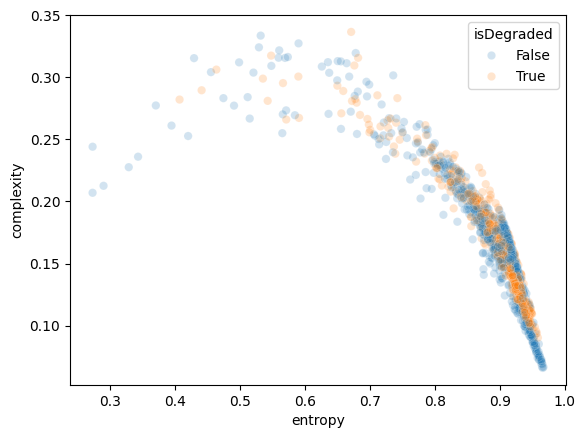
\includegraphics[height=\textheight,width=\textwidth,keepaspectratio]{images/egci_problem_labeled.png}
            \end{column}
            \begin{column}{0.5\textwidth}
                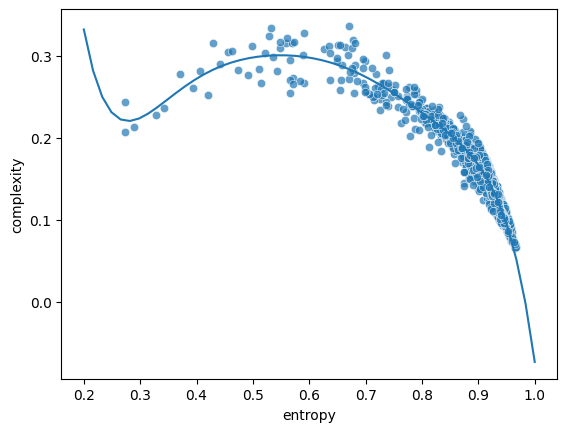
\includegraphics[height=\textheight,width=\textwidth,keepaspectratio]{images/egci_solution.png}
            \end{column}
        \end{columns}
        \caption{EGCI and banding (left), demonstrated solution (right)}
    \end{figure}
\end{frame}
\begin{frame}{EGCI Clustering}
    \centering
    \begin{figure}
        \begin{columns}
            \begin{column}{0.5\textwidth}
                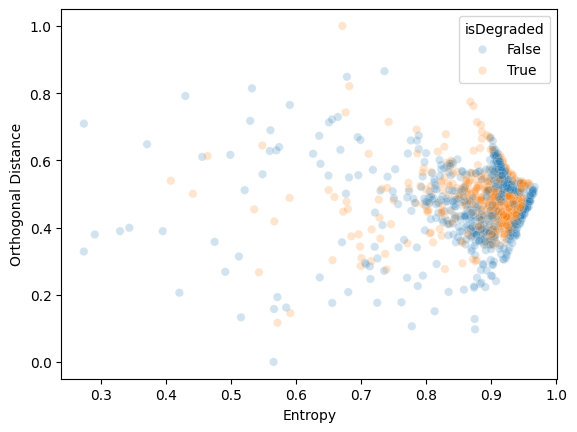
\includegraphics[height=\textheight,width=\textwidth,keepaspectratio]{images/egci_clustering_labeled.png}
            \end{column}
            \begin{column}{0.5\textwidth}
                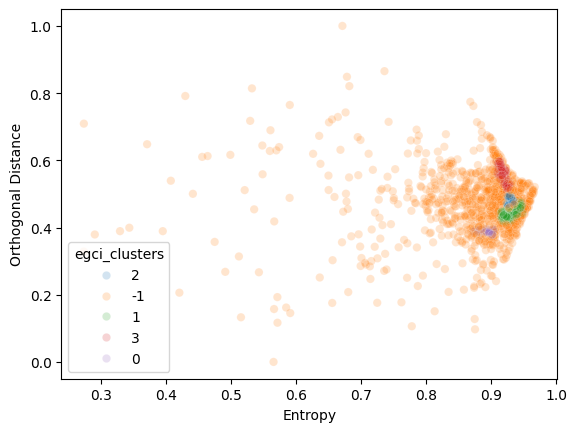
\includegraphics[height=\textheight,width=\textwidth,keepaspectratio]{images/egci_clustering.png}
            \end{column}
        \end{columns}
        \caption{EGCI labeled (left) and with HDBSCAN clusterings (right). \textbf{Note:} the poor clustering, -1 indicates noise
        }
    \end{figure}
\end{frame}

\begin{frame}{Clustering in the Graph}
    \begin{figure}
        \centering
        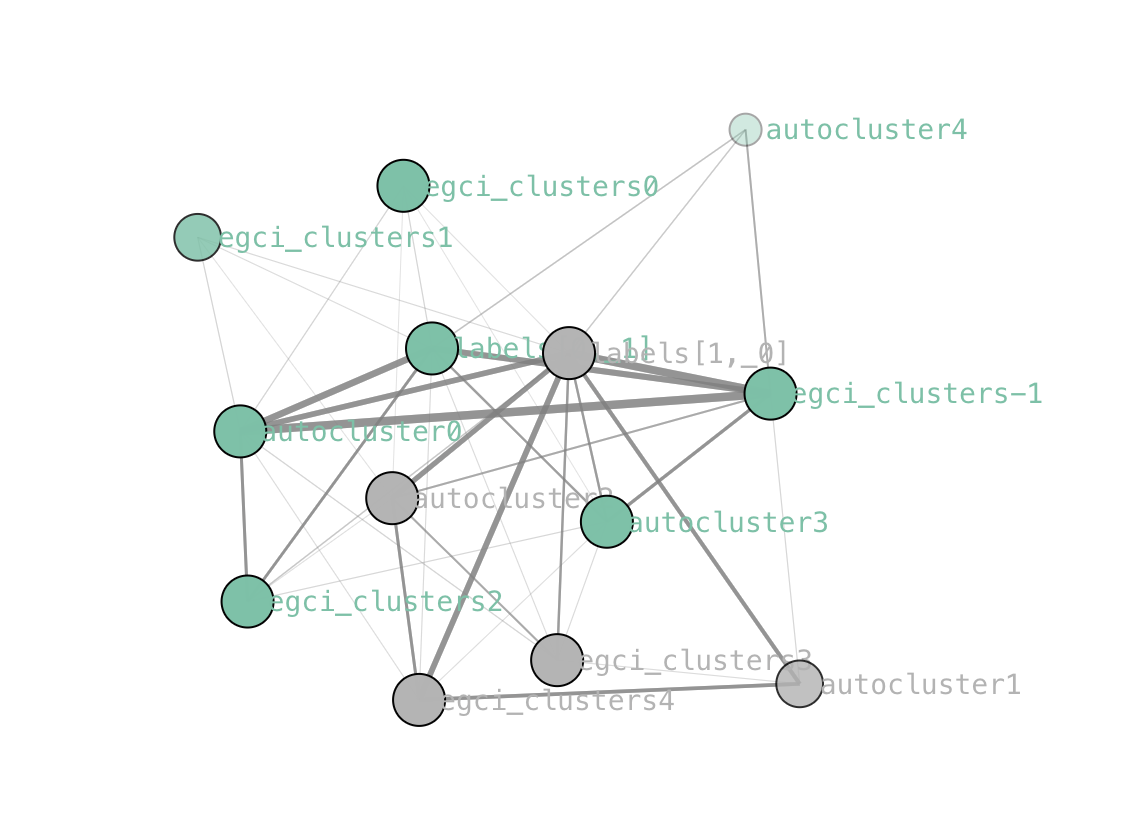
\includegraphics[height=0.7\textheight,width=0.7\textwidth,keepaspectratio]{images/graph_clustering.png}
        \caption{Simple graph with EGCI and autoencoder clustering}
    \end{figure}
    
\end{frame}

\begin{frame}{D3.JS Visualization}
    \begin{itemize}
        \item 
    \end{itemize}
\end{frame}

\begin{frame}{Future Steps}
    \begin{itemize}
        \item 
    \end{itemize}
\end{frame}

\begin{frame}{Collar Team Agenda}
    \begin{itemize}
        \item Integration
        \item Inference Testing
        \item Power Studies
        \item Documentation
        \item Auto Encoders       
    \end{itemize}
\end{frame}

\begin{frame}{Integration}
    \begin{itemize}
        \item Real-Time Clock (RTC) configured
        \item Configuring CM4 core to test power as wake-up system
        \item Noise affecting model inferences → new mic/pipeline bypass
    \end{itemize}
\end{frame}

\begin{frame}{Inference Testing}
    \begin{itemize}
        \item Domain shift from microphone 
        \item Heavy noise in mel bands 20-30, 60, even after filtering
    \end{itemize}
    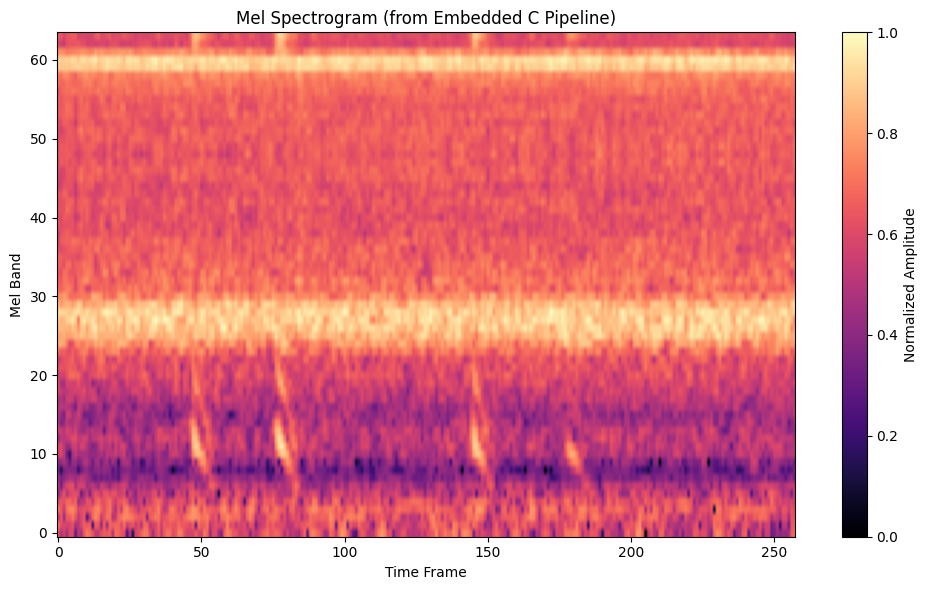
\includegraphics[height=0.7\textheight,width=0.5\textwidth,keepaspectratio]{images/melSpec.png}
    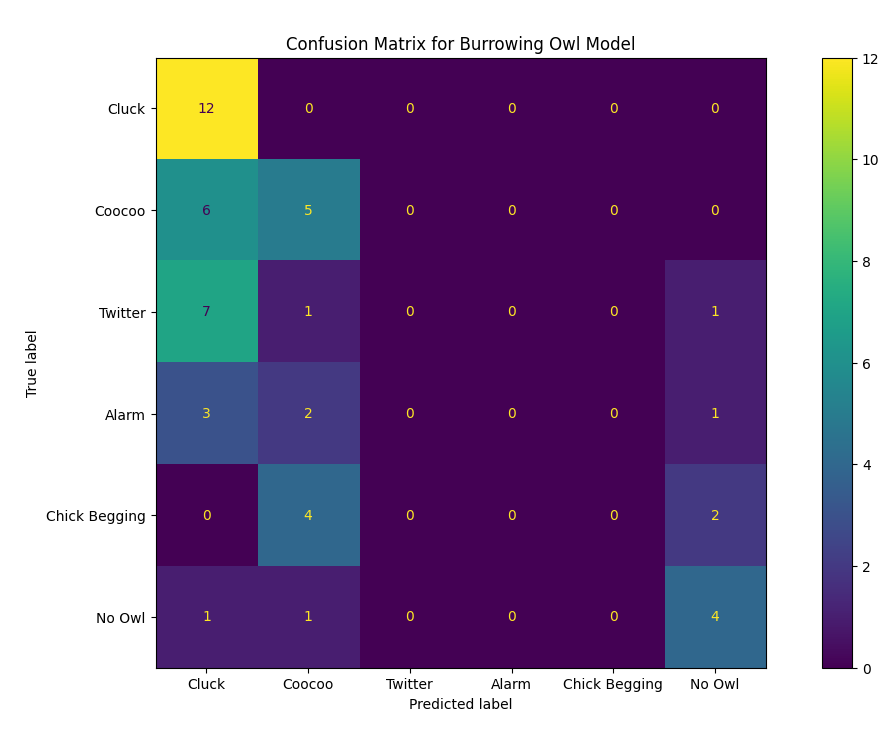
\includegraphics[height=0.7\textheight,width=0.39\textwidth,keepaspectratio]{images/confusionMatrix.png}
\end{frame}

\begin{frame}{Power Studies}
    \begin{itemize}
        \item Testing CM4 core wake-up
        \item Integrated system re-test
        \item Future plans to measure LoRa
    \end{itemize}
    \begin{table}[]
    \begin{tabular}{lll}
    \hline
                & Independent (mA) & Integrated System (mA) \\ \hline
    Baseline       & 13.43            & 6.99                  \\
    Mic            & 23.6             & 10.37                 \\
    Inf + Mel Spec & 16.0             & 12.46                 \\
    MicroSD        & 14.1             & 7.74                  \\
    LoRa          & TBD              & TBD                     \\ \hline
    \end{tabular}
    \end{table}
\end{frame}

\begin{frame}{Documentation}
    \begin{itemize}
        \item Document with erors encountered, design decisions, etc.
        \item Extensive code refactoring, commenting
        \item Embedded Systems Letter
    \end{itemize}
\end{frame}

\begin{frame}{Auto Encoders}
    \begin{itemize}
        \item With max pay load of 222 bytes, roughly 19 packets per recording with current latent space
        \item Next Steps:
        \begin{itemize}
            \item further reduce latent space 
            \item flesh out experiment and test
        \end{itemize}
    \end{itemize}
\end{frame}




